\documentclass{article}
\usepackage{graphicx} % Required for inserting images
\usepackage{float}


\title{24.05.14 Halo2-lib cost and Mithril chain}
\author{Xun Zhang \quad \quad Bingsheng Zhang \\ 
Zhejiang University, CHN \\
22221024@zju.edu.cn \quad bingsheng@zju.edu.cn}

\date{May 14 2024}
\begin{document}

\maketitle

\section{Halo2-lib Group Operation Benchmark}

Following are the benchmark results of group operation in halo2-lib crate.

\begin{table}[H]
    \centering
    \begin{tabular}{p{1cm}|p{1cm}|p{1cm}|p{2cm}|p{1.5cm}|p{1.5cm}|p{1.5cm}|p{1.5cm}} \hline
          degree&advice&lookup&lookup\_bits&limb\_bits&proof\_time&proof\_size&verify\_time \\ \hline
15&10&2&14&88&2.2243s&4128&8.055ms \\ \hline
16&5&1&15&90&2.5095s&2272&7.540ms\\ \hline
17&3&1&16&88&3.8706s&1696&9.775ms\\ \hline
18&2&1&17&88&6.7053s&1344&14.639ms\\ \hline
19&1&0&18&90&11.0751s&960&23.502ms\\ \hline

         
    \end{tabular}
    \caption{Bn254 G2 Addition Cost(Batch size = 100)}
    \label{tab:my_label}
\end{table}


\begin{table}[H]
    \centering
    \begin{tabular}{p{1cm}|p{1cm}|p{1cm}|p{2cm}|p{1.5cm}|p{1.5cm}|p{1.5cm}|p{1.5cm}} \hline
          degree&advice&lookup&lookup\_bits&limb\_bits&proof\_time&proof\_size&verify\_time \\ \hline
16&170&23&15&88&51.5202s&59584&163.06ms \\ \hline
17&84&11&16&88&47.4618s&29120&133.59ms\\ \hline
18&42&6&17&88&49.9059s&15008&135.64ms\\ \hline
19&20&3&18&90&51.1550s&7360&131.00ms\\ \hline
20&11&2&19&90&67.8328s&4128&170.56ms\\ \hline

         
    \end{tabular}
    \caption{Bn254 G2 MSM Cost(Batch size = 100)}
    \label{tab:my_label}
\end{table}


\begin{table}[H]
    \centering
    \begin{tabular}{p{1cm}|p{1cm}|p{1cm}|p{2cm}|p{1.5cm}|p{1.5cm}|p{1.5cm}|p{1.5cm}} \hline
          degree&advice&lookup&lookup\_bits&limb\_bits&proof\_time&proof\_size&verify\_time \\ \hline
14&211&27&13&91&19.5710s&72416&68.38ms \\ \hline
15&105&14&14&90&16.4763s&36416&47.59ms\\ \hline
16&50&6&15&90&14.8747s&17312&48.95ms\\ \hline
17&25&3&16&88&15.2069s&8864&31.46ms\\ \hline
18&13&2&17&88&17.9298s&4928&37.19ms\\ \hline
19&6&1&18&90&20.3571s&2496&38.85ms\\ \hline
20&3&1&19&88&30.7017s&1696&55.82ms\\ \hline
21&2&1&20&88&51.7027s&1344&105.05ms\\ \hline
22&1&1&21&88&91.7061s&960&194.89ms\\ \hline
         
    \end{tabular}
    \caption{Bn254 Pairing Cost}
    \label{tab:my_label}
\end{table}


\section{Signature Verification Proving Time}

Following are the benchmark results of signature verification in halo2-lib and halo2-lib-eddsa crates.


\begin{table}[H]
    \centering
    \begin{tabular}{p{1cm}|p{1cm}|p{1cm}|p{2cm}|p{1.5cm}|p{1.5cm}|p{1.5cm}|p{1.5cm}} \hline
          degree&advice&lookup&lookup\_bits&limb\_bits&proof\_time&proof\_size&verify\_time \\ \hline
14&211&27&13&91&25.3671s&95808&119.31ms \\ \hline
15&105&14&14&90&22.8869s&48000&63.41ms\\ \hline
16&50&6&15&90&20.6673s&22752&54.23ms\\ \hline
17&25&3&16&88&20.4768s&11520&50.50ms\\ \hline
18&13&2&17&88&22.5167s&6080&52.44ms\\ \hline
19&6&1&18&90&24.9818s&3072&56.68ms\\ \hline
20&3&1&19&88&36.0663s&1920&85.64ms\\ \hline
21&2&1&20&88&56.5497s&1344&125.96ms\\ \hline
    \end{tabular}
    \caption{Bn254 BLS Signature Verification Cost}
    \label{tab:my_label}
\end{table}


\begin{table}[H]
    \centering
    \begin{tabular}{p{1cm}|p{1cm}|p{1cm}|p{2cm}|p{1.5cm}|p{1.5cm}|p{1.5cm}|p{1.5cm}} \hline
          degree&advice&lookup&lookup\_bits&limb\_bits&proof\_time&proof\_size&verify\_time \\ \hline
19&1&1&18&88&11.7409s&960&20.68ms \\ \hline
18&2&1&17&88&7.1555s&1344&16.03ms\\ \hline
17&4&1&16&88&4.4740s&1920&10.86ms\\ \hline
16&8&2&15&90&3.9142s&3776&11.29ms\\ \hline
15&17&3&14&90&3.5269s&6784&12.91ms\\ \hline
14&34&6&13&91&3.8446s&13984&17.18ms\\ \hline
13&68&12&12&88&4.4652s&27072&30.02ms\\ \hline

    \end{tabular}
    \caption{Secp256k1 ECDSA Signature Verification Cost}
    \label{tab:my_label}
\end{table}


\begin{table}[H]
    \centering
    \begin{tabular}{p{1cm}|p{1cm}|p{1cm}|p{2cm}|p{1.5cm}|p{1.5cm}|p{1.5cm}|p{1.5cm}} \hline
          degree&advice&lookup&lookup\_bits&limb\_bits&proof\_time&proof\_size&verify\_time \\ \hline
19&1&1&18&88&17.4019s&1920&28.54ms  \\ \hline
18&2&1&17&88&13.1093s&3200&24.94ms \\ \hline
17&4&1&16&88&11.4594s&5632&22.69ms \\ \hline
16&8&2&15&90&10.1348s&10976&25.03ms \\ \hline
15&17&3&14&90&10.7261s&22688&37.71ms \\ \hline
14&34&6&13&91&12.2806s&46240&49.46ms \\ \hline
13&68&12&12&88&15.4048s&94048&82.81ms \\ \hline


    \end{tabular}
    \caption{ED25519 EDDSA Signature Verification Cost}
    \label{tab:my_label}
\end{table}


\section{Mithril Certificate Chain}

\subsection{Certificate Chain Introduction}

The \textbf{certificate chain} is a Mithril component that certifies the \textbf{stake distribution} used to create the multi-signature. Its primary purpose is to prevent adversaries from executing an \textbf{eclipse attack} on the blockchain.

Without the certificate, the stake distribution can't be trusted. A malicious actor could relatively easily create a fake stake distribution and use it to produce a valid multi-signature, which would be embedded in a valid but non-genuine certificate. This certificate could be served by a dishonest Mithril aggregator node, leading an honest Mithril client to restore a non-genuine snapshot.


The way to certify the stake distribution used to create a multi-signature is by verifying that it has been previously signed in an earlier certificate. Then, one can recursively verify that the earlier certificate is valid in the same manner. This process can be structured as a chain of certificates, known as the Mithril certificate chain. The first certificate in the chain is discussed below.


Since multiple certificates can be created during the same epoch using the same stake distribution, it is not necessary to link to all of them for verification. Instead, it is sufficient to link to only one certificate from the previous epoch. By doing so, the verification process becomes faster and helps avoid network congestion.


The first certificate in the certificate chain is known as the genesis certificate. Validating the stake distribution embedded in the genesis certificate is only possible by signing it with a private key linked to a widely accessible public key called the genesis key. The use of these specific keys ensures the integrity and security of the initial stake distribution and subsequent transitions within the blockchain network.

The diagram below presents the certificate chain design:


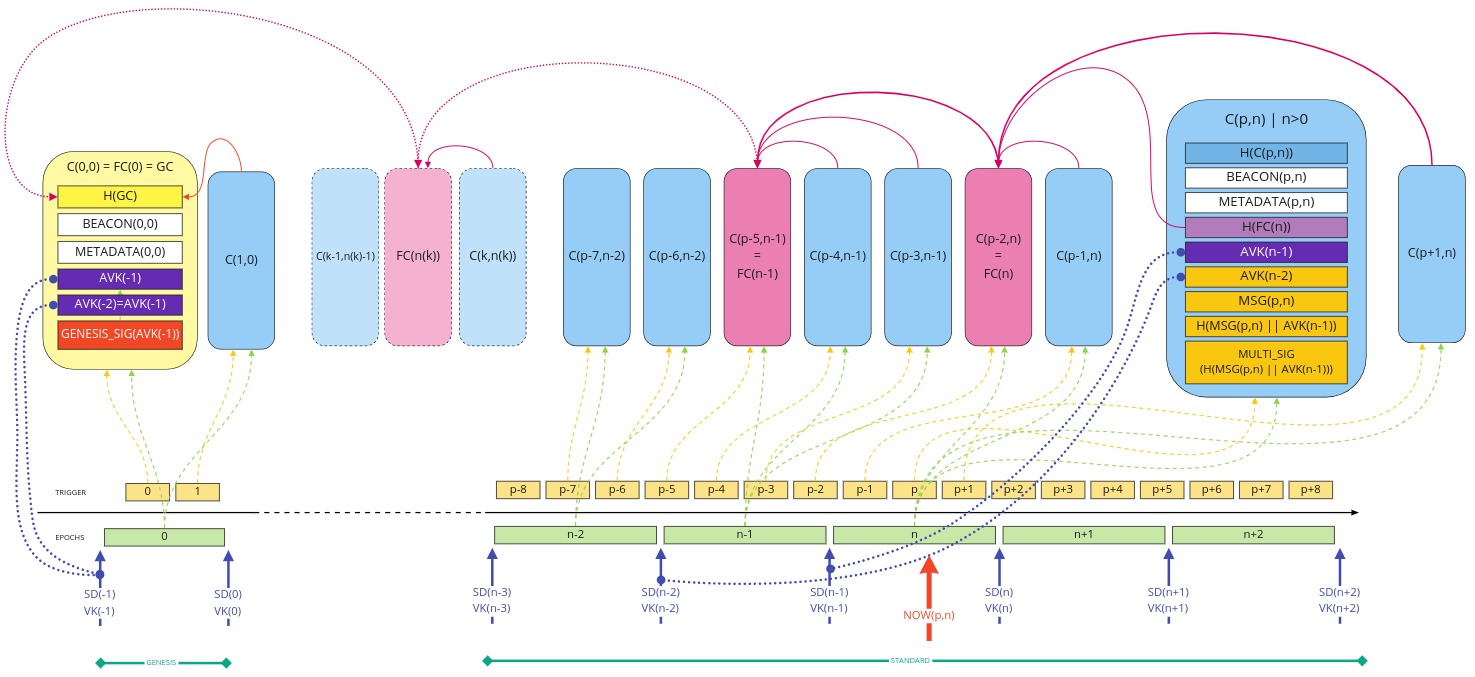
\includegraphics[width=1\linewidth]{certificate-chain-e700241394649f948e0aab47b0f881c9.jpg}

Where the following notations have been used:

\begin{itemize}
    \item C(p,n): Certificate at trigger p and epoch n
\item FC(n): First certificate of epoch n
\item GC: Genesis certificate
\item H(): Hash
\item SD(n): Stake distribution of epoch n
\item VK(n): Verification key at epoch n
\item AVK(n): Aggregrate verification key at epoch n such as $AVK(n) = MKT\_ROOT(SD(n)\vert\vert VK(n))$
\item MKT\_ROOT(): Merkle-tree root
\item BEACON(p,n): Beacon at trigger p and epoch n
\item METADATA(p,n): Metadata of the certificate at trigger p and epoch n
\item MSG(p,n): Message of the certificate at trigger p and epoch n
\item MULTI\_SIG(p,n): Multi-signature created to the message $H(MSG(p,n) \vert \vert AVK(n-1))$
\end{itemize}

\subsection{How to Validate a Certificate Chain}

The \textbf{aggregate verification key (AVK)} is the root of the Merkle tree where each leaf is filled with $H(STAKE(signer) \vert \vert VK(signer))$. It represents the corresponding stake distribution in a condensed way.

\begin{itemize}
    \item To validate a \textbf{certificate chain}: a least a valid certificate per epoch.
    \item To validate a \textbf{non-genesis certificate}: iff the AVK used to verify the multi-signature is also part of the signed message used to create a valid multi-signature in a previously sealed certificate. 
    \item To validate a \textbf{genesis certificate}: iff its genesis signature is verified with the advertised public genesis key.
\end{itemize}

An implementation of the algorithm would work as follows for a certificate:
\begin{itemize}
    \item \textbf{Step 1}: Use this certificate as $\mathsf{current\_certificate}$.
    \item \textbf{Step 2}: Verify (or fail) that the $\mathsf{current\_hash}$ of the $\mathsf{current\_certificate}$ is valid by computing it and comparing it with the $\mathsf{hash}$ field of the certificate.
    \item \textbf{Step 3}: Get the $\mathsf{previous\_hash}$ of the $\mathsf{previous\_certificate}$ by reading its value in the $\mathsf{current\_certificate}$.
    \item \textbf{Step 4}: Verify (or fail) that the $\mathsf{multi\_signature}$ of the $\mathsf{current\_certificate}$ is valid.
    \item \textbf{Step 5}: Retrieve the $\mathsf{previous\_certificate}$ that has the hash $\mathsf{previous\_hash}$.
        \begin{itemize}
            \item \textbf{Step 5.1}: If it is not a $\mathsf{genesis\_certificate}$:

            \begin{itemize}
                \item \textbf{Step 5.1.1}: Verify (or fail) that the $\mathsf{previous\_hash}$ of the $\mathsf{previous\_certificate}$ is valid by computing it and comparing it with the $\mathsf{hash}$ field of the certificate.
                \item \textbf{Step 5.1.2}: Verify the $\mathsf{current\_avk}$:

                \begin{itemize}
                    \item \textbf{Step 5.1.2.1}: If the $\mathsf{current\_certificate}$ is the $\mathsf{first\_certificate}$ of the epoch, verify (or fail) that the $\mathsf{current\_avk}$ of the $\mathsf{current\_certificate}$ is part of the message signed by the multi-signature of the $\mathsf{previous\_certificate}$.
                    \item \textbf{Step 5.1.2.2}: Else verify (or fail) that the $\mathsf{current\_avk}$ of the $\mathsf{current\_certificate}$ is the same as the  $\mathsf{current\_avk}$ of the $\mathsf{previous\_certificate}$.
                \end{itemize}

                \item \textbf{Step 5.1.3}: Verify (or fail) that the $\mathsf{multi\_signature}$ of the $\mathsf{previous\_certificate}$ is valid .

                \item \textbf{Step 5.1.4}: Use the $\mathsf{previous\_certificate}$ as $\mathsf{current\_certificate}$ and start again at \textbf{Step 2}.

                
            \end{itemize}

        \item \textbf{Step 5.2}: If it is a $\mathsf{genesis\_certificate}$:
            \begin{itemize}
                \item \textbf{Step 5.2.1}: Verify (or fail) that the $\mathsf{previous\_hash}$ of the $\mathsf{previous\_certificate}$ is valid by computing it and comparing it with the $\mathsf{hash}$ field of the certificate.
                \item \textbf{Step 5.2.2}: Verify (or fail) that the $\mathsf{current\_avk}$ of the $\mathsf{current\_certificate}$ is part of the message signed by the genesis signature of the $\mathsf{previous\_certificate}$.
                \item \textbf{Step 5.2.3}: The certificate is valid (success).
            \end{itemize}
        \end{itemize}
\end{itemize}

\subsection{The coexistence of multiple certificate chains}

What would happen if some Mithril aggregator claims that not enough signatures were received? This doesn’t really matter, as there will be a different Mithril aggregator that would collect sufficient signatures and aggregate them into a valid certificate.

Similarly, different Mithril aggregators might have different views of the individual signatures submitted (one aggregator might receive 10 signatures, and a different one could receive 11), which would result in different certificates signing the same message.

This would result in different certificate chains that would all link back to the genesis certificate. Indeed they would be represented by a tree of certificates where each traversal path from the root to a leaf represents a valid certificate chain.


\end{document}
